\section{Compiling Toffoli Gates}
\label{sec:elbows}


\begin{figure}
    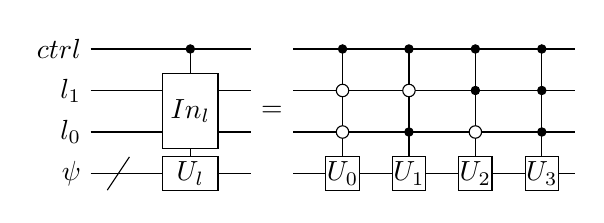
\begin{tikzpicture}[scale=1.000000,x=1pt,y=1pt]
\filldraw[color=white] (0.000000, -7.500000) rectangle (175.000000, 52.500000);
% Drawing wires
% Line 1: ctrl W ctrl
\draw[color=black] (0.000000,45.000000) -- (175.000000,45.000000);
\draw[color=black] (0.000000,45.000000) node[left] {$ctrl$};
% Line 2: l1 W l_1
\draw[color=black] (0.000000,30.000000) -- (175.000000,30.000000);
\draw[color=black] (0.000000,30.000000) node[left] {$l_1$};
% Line 3: l0 W l_0
\draw[color=black] (0.000000,15.000000) -- (175.000000,15.000000);
\draw[color=black] (0.000000,15.000000) node[left] {$l_0$};
% Line 4: sys W \psi
\draw[color=black] (0.000000,0.000000) -- (175.000000,0.000000);
\draw[color=black] (0.000000,0.000000) node[left] {$\psi$};
% Done with wires; drawing gates
% Line 6: sys /
\draw (6.000000, -6.000000) -- (14.000000, 6.000000);
% Line 8: l0 l1 G width=20  $In_l$ sys G width=20 $U_l$ ctrl
\draw (36.000000,45.000000) -- (36.000000,0.000000);
\begin{scope}
\draw[fill=white] (36.000000, 22.500000) +(-45.000000:14.142136pt and 19.091883pt) -- +(45.000000:14.142136pt and 19.091883pt) -- +(135.000000:14.142136pt and 19.091883pt) -- +(225.000000:14.142136pt and 19.091883pt) -- cycle;
\clip (36.000000, 22.500000) +(-45.000000:14.142136pt and 19.091883pt) -- +(45.000000:14.142136pt and 19.091883pt) -- +(135.000000:14.142136pt and 19.091883pt) -- +(225.000000:14.142136pt and 19.091883pt) -- cycle;
\draw (36.000000, 22.500000) node {$In_l$};
\end{scope}
\begin{scope}
\draw[fill=white] (36.000000, -0.000000) +(-45.000000:14.142136pt and 8.485281pt) -- +(45.000000:14.142136pt and 8.485281pt) -- +(135.000000:14.142136pt and 8.485281pt) -- +(225.000000:14.142136pt and 8.485281pt) -- cycle;
\clip (36.000000, -0.000000) +(-45.000000:14.142136pt and 8.485281pt) -- +(45.000000:14.142136pt and 8.485281pt) -- +(135.000000:14.142136pt and 8.485281pt) -- +(225.000000:14.142136pt and 8.485281pt) -- cycle;
\draw (36.000000, -0.000000) node {$U_l$};
\end{scope}
\filldraw (36.000000, 45.000000) circle(1.500000pt);
% Line 10: =
\draw[fill=white,color=white] (58.000000, -6.000000) rectangle (73.000000, 51.000000);
\draw (65.500000, 22.500000) node {$=$};
% Line 12: sys G $U_0$ -l0 -l1 ctrl
\draw (91.000000,45.000000) -- (91.000000,0.000000);
\begin{scope}
\draw[fill=white] (91.000000, -0.000000) +(-45.000000:8.485281pt and 8.485281pt) -- +(45.000000:8.485281pt and 8.485281pt) -- +(135.000000:8.485281pt and 8.485281pt) -- +(225.000000:8.485281pt and 8.485281pt) -- cycle;
\clip (91.000000, -0.000000) +(-45.000000:8.485281pt and 8.485281pt) -- +(45.000000:8.485281pt and 8.485281pt) -- +(135.000000:8.485281pt and 8.485281pt) -- +(225.000000:8.485281pt and 8.485281pt) -- cycle;
\draw (91.000000, -0.000000) node {$U_0$};
\end{scope}
\draw[fill=white] (91.000000, 15.000000) circle(2.250000pt);
\draw[fill=white] (91.000000, 30.000000) circle(2.250000pt);
\filldraw (91.000000, 45.000000) circle(1.500000pt);
% Line 13: sys G $U_1$ l0 -l1 ctrl
\draw (115.000000,45.000000) -- (115.000000,0.000000);
\begin{scope}
\draw[fill=white] (115.000000, -0.000000) +(-45.000000:8.485281pt and 8.485281pt) -- +(45.000000:8.485281pt and 8.485281pt) -- +(135.000000:8.485281pt and 8.485281pt) -- +(225.000000:8.485281pt and 8.485281pt) -- cycle;
\clip (115.000000, -0.000000) +(-45.000000:8.485281pt and 8.485281pt) -- +(45.000000:8.485281pt and 8.485281pt) -- +(135.000000:8.485281pt and 8.485281pt) -- +(225.000000:8.485281pt and 8.485281pt) -- cycle;
\draw (115.000000, -0.000000) node {$U_1$};
\end{scope}
\filldraw (115.000000, 15.000000) circle(1.500000pt);
\draw[fill=white] (115.000000, 30.000000) circle(2.250000pt);
\filldraw (115.000000, 45.000000) circle(1.500000pt);
% Line 14: sys G $U_2$ -l0 l1 ctrl
\draw (139.000000,45.000000) -- (139.000000,0.000000);
\begin{scope}
\draw[fill=white] (139.000000, -0.000000) +(-45.000000:8.485281pt and 8.485281pt) -- +(45.000000:8.485281pt and 8.485281pt) -- +(135.000000:8.485281pt and 8.485281pt) -- +(225.000000:8.485281pt and 8.485281pt) -- cycle;
\clip (139.000000, -0.000000) +(-45.000000:8.485281pt and 8.485281pt) -- +(45.000000:8.485281pt and 8.485281pt) -- +(135.000000:8.485281pt and 8.485281pt) -- +(225.000000:8.485281pt and 8.485281pt) -- cycle;
\draw (139.000000, -0.000000) node {$U_2$};
\end{scope}
\draw[fill=white] (139.000000, 15.000000) circle(2.250000pt);
\filldraw (139.000000, 30.000000) circle(1.500000pt);
\filldraw (139.000000, 45.000000) circle(1.500000pt);
% Line 15: sys G $U_3$ l0 l1 ctrl
\draw (163.000000,45.000000) -- (163.000000,0.000000);
\begin{scope}
\draw[fill=white] (163.000000, -0.000000) +(-45.000000:8.485281pt and 8.485281pt) -- +(45.000000:8.485281pt and 8.485281pt) -- +(135.000000:8.485281pt and 8.485281pt) -- +(225.000000:8.485281pt and 8.485281pt) -- cycle;
\clip (163.000000, -0.000000) +(-45.000000:8.485281pt and 8.485281pt) -- +(45.000000:8.485281pt and 8.485281pt) -- +(135.000000:8.485281pt and 8.485281pt) -- +(225.000000:8.485281pt and 8.485281pt) -- cycle;
\draw (163.000000, -0.000000) node {$U_3$};
\end{scope}
\filldraw (163.000000, 15.000000) circle(1.500000pt);
\filldraw (163.000000, 30.000000) circle(1.500000pt);
\filldraw (163.000000, 45.000000) circle(1.500000pt);
% Done with gates; drawing ending labels
% Done with ending labels; drawing cut lines and comments
% Done with comments
\end{tikzpicture}

    \caption{
        \textbf{Uniformly Controlled Operations}
        A series of operations that are subsequently controlled on the computational basis states of a register are referred to as \textit{uniformly controlled operations}.
    }
    \label{fig:uniformly-controlled-ops}
\end{figure}


\begin{figure*}
    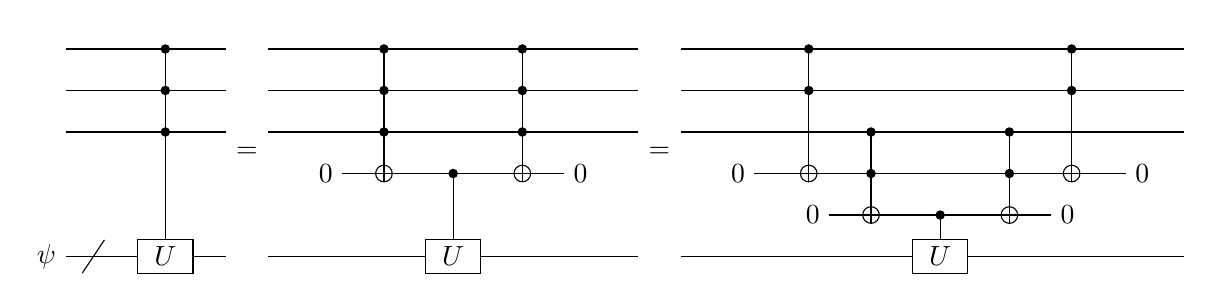
\begin{tikzpicture}[scale=1.000000,x=1pt,y=1pt]
\filldraw[color=white] (0.000000, -7.500000) rectangle (404.000000, 82.500000);
% Drawing wires
% Line 1: 0 W
\draw[color=black] (0.000000,75.000000) -- (404.000000,75.000000);
% Line 2: 1 W
\draw[color=black] (0.000000,60.000000) -- (404.000000,60.000000);
% Line 3: 2 W
\draw[color=black] (0.000000,45.000000) -- (404.000000,45.000000);
% Line 4: c0 W 0 0 0 0
\draw[color=black] (92.500000,30.000000) -- (187.500000,30.000000);
\draw[color=black] (241.500000,30.000000) -- (390.500000,30.000000);
% Line 5: c1 W 0 0
\draw[color=black] (268.500000,15.000000) -- (363.500000,15.000000);
% Line 6: sys W \psi
\draw[color=black] (0.000000,0.000000) -- (404.000000,0.000000);
\draw[color=black] (0.000000,0.000000) node[left] {$\psi$};
% Done with wires; drawing gates
% Line 8: sys /
\draw (6.000000, -6.000000) -- (14.000000, 6.000000);
% Line 10: sys G width=20 $U$ 0 1 2
\draw (36.000000,75.000000) -- (36.000000,0.000000);
\begin{scope}
\draw[fill=white] (36.000000, -0.000000) +(-45.000000:14.142136pt and 8.485281pt) -- +(45.000000:14.142136pt and 8.485281pt) -- +(135.000000:14.142136pt and 8.485281pt) -- +(225.000000:14.142136pt and 8.485281pt) -- cycle;
\clip (36.000000, -0.000000) +(-45.000000:14.142136pt and 8.485281pt) -- +(45.000000:14.142136pt and 8.485281pt) -- +(135.000000:14.142136pt and 8.485281pt) -- +(225.000000:14.142136pt and 8.485281pt) -- cycle;
\draw (36.000000, -0.000000) node {$U$};
\end{scope}
\filldraw (36.000000, 75.000000) circle(1.500000pt);
\filldraw (36.000000, 60.000000) circle(1.500000pt);
\filldraw (36.000000, 45.000000) circle(1.500000pt);
% Line 12: =
\draw[fill=white,color=white] (58.000000, -6.000000) rectangle (73.000000, 81.000000);
\draw (65.500000, 37.500000) node {$=$};
% Line 14: c0 START
\draw[color=black] (100.000000,30.000000) node[fill=white,left,minimum height=15.000000pt,minimum width=15.000000pt,inner sep=0pt] {\phantom{$0$}};
\draw[color=black] (100.000000,30.000000) node[left] {$0$};
% Line 15: 0 1 2 +c0
\draw (115.000000,75.000000) -- (115.000000,30.000000);
\filldraw (115.000000, 75.000000) circle(1.500000pt);
\filldraw (115.000000, 60.000000) circle(1.500000pt);
\filldraw (115.000000, 45.000000) circle(1.500000pt);
\begin{scope}
\draw[fill=white] (115.000000, 30.000000) circle(3.000000pt);
\clip (115.000000, 30.000000) circle(3.000000pt);
\draw (112.000000, 30.000000) -- (118.000000, 30.000000);
\draw (115.000000, 27.000000) -- (115.000000, 33.000000);
\end{scope}
% Line 16: sys G width=20 $U$ c0
\draw (140.000000,30.000000) -- (140.000000,0.000000);
\begin{scope}
\draw[fill=white] (140.000000, -0.000000) +(-45.000000:14.142136pt and 8.485281pt) -- +(45.000000:14.142136pt and 8.485281pt) -- +(135.000000:14.142136pt and 8.485281pt) -- +(225.000000:14.142136pt and 8.485281pt) -- cycle;
\clip (140.000000, -0.000000) +(-45.000000:14.142136pt and 8.485281pt) -- +(45.000000:14.142136pt and 8.485281pt) -- +(135.000000:14.142136pt and 8.485281pt) -- +(225.000000:14.142136pt and 8.485281pt) -- cycle;
\draw (140.000000, -0.000000) node {$U$};
\end{scope}
\filldraw (140.000000, 30.000000) circle(1.500000pt);
% Line 17: 0 1 2 +c0
\draw (165.000000,75.000000) -- (165.000000,30.000000);
\filldraw (165.000000, 75.000000) circle(1.500000pt);
\filldraw (165.000000, 60.000000) circle(1.500000pt);
\filldraw (165.000000, 45.000000) circle(1.500000pt);
\begin{scope}
\draw[fill=white] (165.000000, 30.000000) circle(3.000000pt);
\clip (165.000000, 30.000000) circle(3.000000pt);
\draw (162.000000, 30.000000) -- (168.000000, 30.000000);
\draw (165.000000, 27.000000) -- (165.000000, 33.000000);
\end{scope}
% Line 18: c0 END
\draw[color=black] (180.000000,30.000000) node[fill=white,right,minimum height=15.000000pt,minimum width=15.000000pt,inner sep=0pt] {\phantom{$0$}};
\draw[color=black] (180.000000,30.000000) node[right] {$0$};
% Line 20: =
\draw[fill=white,color=white] (207.000000, -6.000000) rectangle (222.000000, 81.000000);
\draw (214.500000, 37.500000) node {$=$};
% Line 22: c0 START
\draw[color=black] (249.000000,30.000000) node[fill=white,left,minimum height=15.000000pt,minimum width=15.000000pt,inner sep=0pt] {\phantom{$0$}};
\draw[color=black] (249.000000,30.000000) node[left] {$0$};
% Line 23: 0 1 +c0
\draw (268.500000,75.000000) -- (268.500000,30.000000);
\filldraw (268.500000, 75.000000) circle(1.500000pt);
\filldraw (268.500000, 60.000000) circle(1.500000pt);
\begin{scope}
\draw[fill=white] (268.500000, 30.000000) circle(3.000000pt);
\clip (268.500000, 30.000000) circle(3.000000pt);
\draw (265.500000, 30.000000) -- (271.500000, 30.000000);
\draw (268.500000, 27.000000) -- (268.500000, 33.000000);
\end{scope}
% Line 24: c1 START
\draw[color=black] (276.000000,15.000000) node[fill=white,left,minimum height=15.000000pt,minimum width=15.000000pt,inner sep=0pt] {\phantom{$0$}};
\draw[color=black] (276.000000,15.000000) node[left] {$0$};
% Line 25: c0 2 +c1
\draw (291.000000,45.000000) -- (291.000000,15.000000);
\filldraw (291.000000, 30.000000) circle(1.500000pt);
\filldraw (291.000000, 45.000000) circle(1.500000pt);
\begin{scope}
\draw[fill=white] (291.000000, 15.000000) circle(3.000000pt);
\clip (291.000000, 15.000000) circle(3.000000pt);
\draw (288.000000, 15.000000) -- (294.000000, 15.000000);
\draw (291.000000, 12.000000) -- (291.000000, 18.000000);
\end{scope}
% Line 26: sys G width=20 $U$ c1
\draw (316.000000,15.000000) -- (316.000000,0.000000);
\begin{scope}
\draw[fill=white] (316.000000, -0.000000) +(-45.000000:14.142136pt and 8.485281pt) -- +(45.000000:14.142136pt and 8.485281pt) -- +(135.000000:14.142136pt and 8.485281pt) -- +(225.000000:14.142136pt and 8.485281pt) -- cycle;
\clip (316.000000, -0.000000) +(-45.000000:14.142136pt and 8.485281pt) -- +(45.000000:14.142136pt and 8.485281pt) -- +(135.000000:14.142136pt and 8.485281pt) -- +(225.000000:14.142136pt and 8.485281pt) -- cycle;
\draw (316.000000, -0.000000) node {$U$};
\end{scope}
\filldraw (316.000000, 15.000000) circle(1.500000pt);
% Line 27: c0 2 +c1
\draw (341.000000,45.000000) -- (341.000000,15.000000);
\filldraw (341.000000, 30.000000) circle(1.500000pt);
\filldraw (341.000000, 45.000000) circle(1.500000pt);
\begin{scope}
\draw[fill=white] (341.000000, 15.000000) circle(3.000000pt);
\clip (341.000000, 15.000000) circle(3.000000pt);
\draw (338.000000, 15.000000) -- (344.000000, 15.000000);
\draw (341.000000, 12.000000) -- (341.000000, 18.000000);
\end{scope}
% Line 28: c1 END
\draw[color=black] (356.000000,15.000000) node[fill=white,right,minimum height=15.000000pt,minimum width=15.000000pt,inner sep=0pt] {\phantom{$0$}};
\draw[color=black] (356.000000,15.000000) node[right] {$0$};
% Line 29: 0 1 +c0
\draw (363.500000,75.000000) -- (363.500000,30.000000);
\filldraw (363.500000, 75.000000) circle(1.500000pt);
\filldraw (363.500000, 60.000000) circle(1.500000pt);
\begin{scope}
\draw[fill=white] (363.500000, 30.000000) circle(3.000000pt);
\clip (363.500000, 30.000000) circle(3.000000pt);
\draw (360.500000, 30.000000) -- (366.500000, 30.000000);
\draw (363.500000, 27.000000) -- (363.500000, 33.000000);
\end{scope}
% Line 30: c0 END
\draw[color=black] (383.000000,30.000000) node[fill=white,right,minimum height=15.000000pt,minimum width=15.000000pt,inner sep=0pt] {\phantom{$0$}};
\draw[color=black] (383.000000,30.000000) node[right] {$0$};
% Done with gates; drawing ending labels
% Done with ending labels; drawing cut lines and comments
% Done with comments
\end{tikzpicture}

    \caption{
        \textbf{Multi-Controlled Operations}
        Operations with multiple controls are referred to as \textit{multi-controlled operations}.
        An $N$-controlled operation can be decomposed into $2(N-2)$ Toffoli gates using $N-1$ clean ancillae.
    }
    \label{fig:multi-controlled-op}
\end{figure*}


The Toffoli gate is a ubiquitous operation in quantum algorithms and is often a significant contributor to the number of non-Clifford resources.
In many algorithms - including those described in this work - a series of Toffoli gates are used to perform an operation that is coherently controlled on the logical-AND of several variables (Figure \ref{fig:multi-controlled-op}).
Therefore, even small reductions in the cost of compiling a Toffoli gate can have a significant impact on the overall spacetime cost of an algorithm.
In an effort to keep this work self-contained, we review a specific compilation technique that can reduce the number of T gates required to synthesize a pair of $N$-controlled Toffoli gates. 

In Nielsen and Chuang \cite{nielsen2001quantum}, a method for synthesizing a single Toffoli gate from $7$ T gates is shown which is likely derived from the methods proposed by Barenco et al. \cite{barenco1995elementary}.
Selinger \cite{selinger2013quantum} and Jones \cite{jones2013low} reduce this cost for a single Toffoli gate from $7$ T gates to $4$ using one clean ancilla.
To the best of our knowledge, this is the most T-gate efficient compilation for a single Toffoli gate.


\begin{figure}
    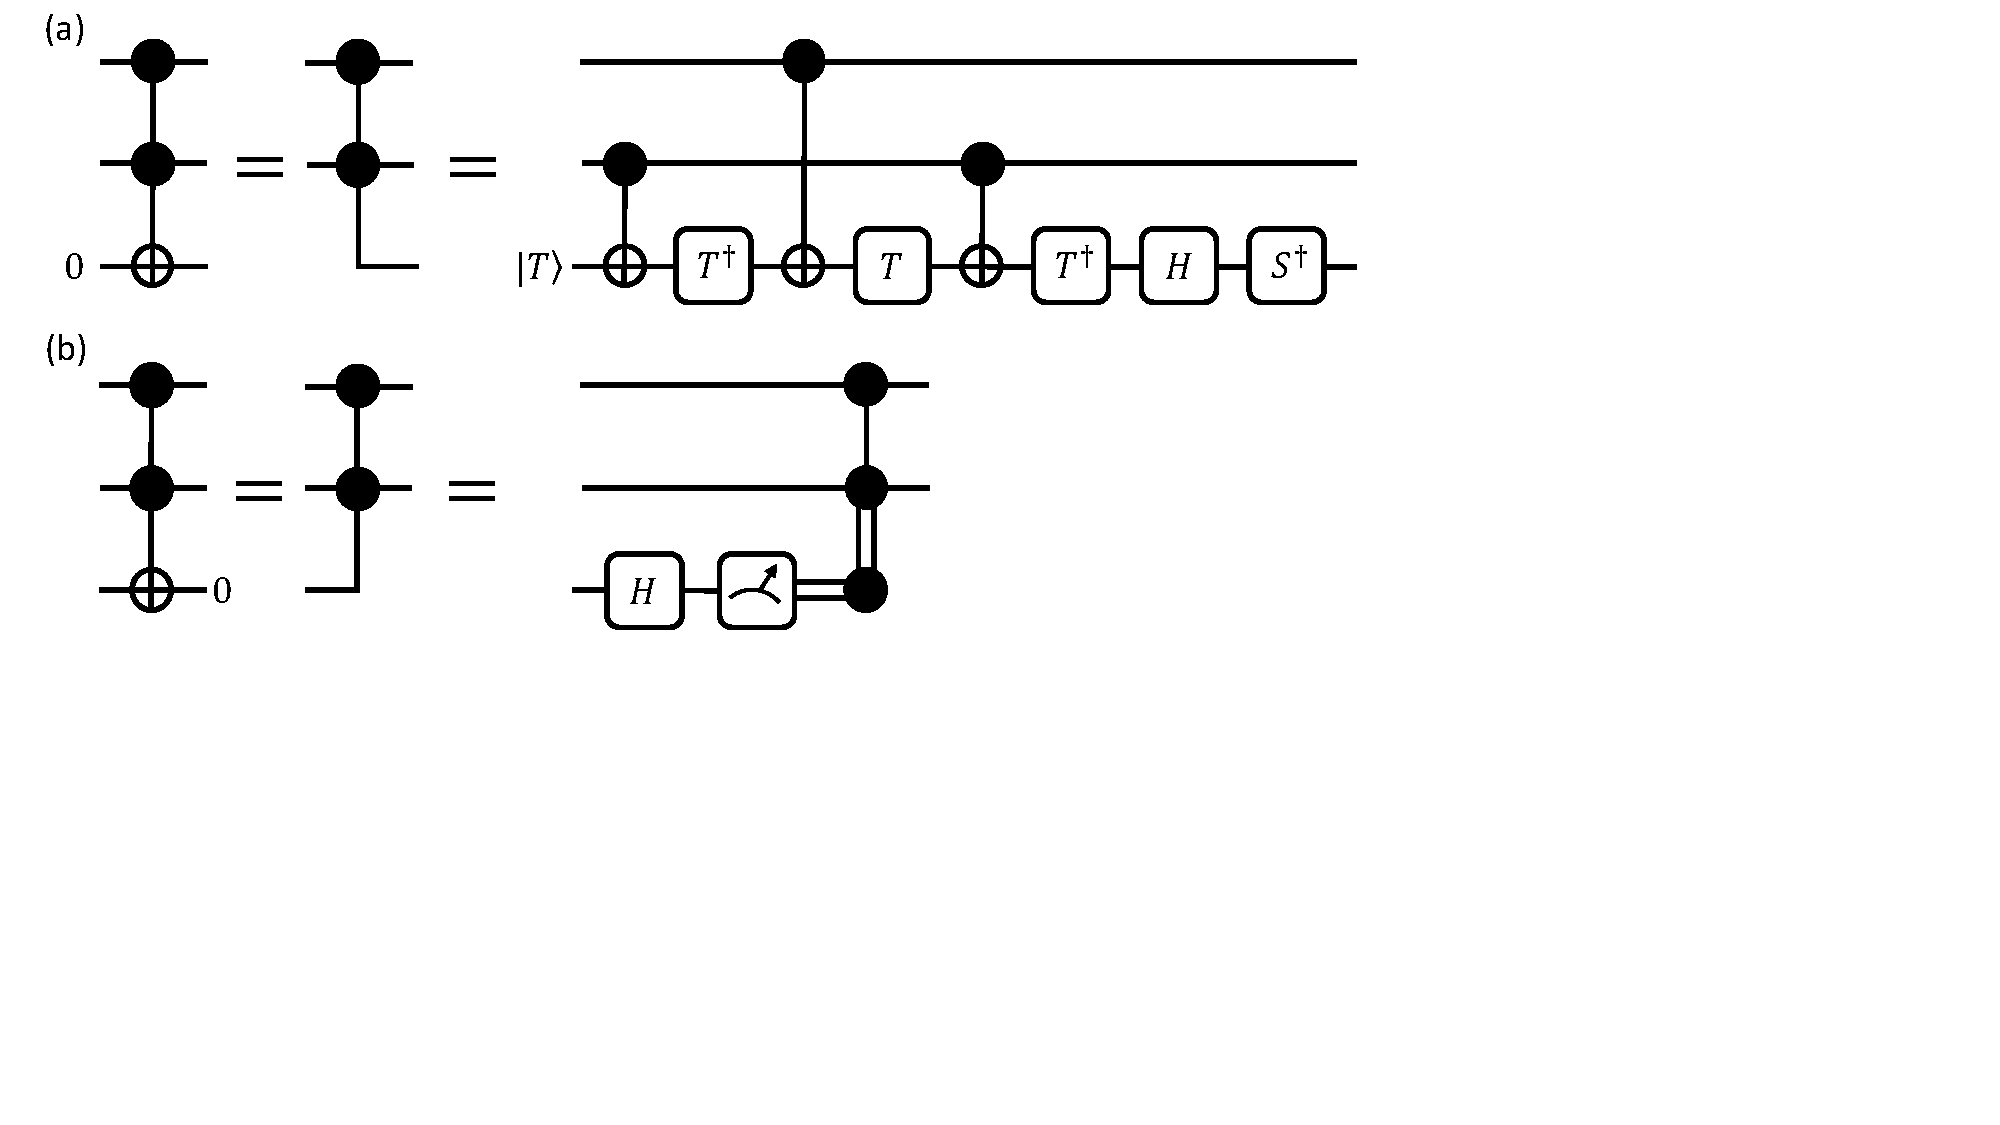
\includegraphics[width=8cm]{figures/elbows}
    \caption{
        \textbf{Elbows}
        In (a), a compilation scheme for a Toffoli gate acting on a clean ancillae is shown that uses four T gates.
        This is sometimes referred to as a ``left-elbow''.
        In (b), a compilation scheme for a Toffoli gate that uncomputes a clean ancillae is shown that uses a measurement and classically conditioned operation.
        This is sometimes referred to as a ``right-elbow''.
    }
    \label{fig:elbows}
\end{figure}

Gidney \cite{gidney2018halving} showed that a pair of Toffoli gates which subsequently compute and uncompute the logical-AND of two variables can be synthesized using $4$ T gates, a measurement, and a classically conditioned operation (Figure 3 of \cite{gidney2018halving}).
This compilation scheme is sometimes referred to as ``elbows'' and is depicted in Figure \ref{fig:elbows}.

Following the methods shown by Barenco et al. \cite{barenco1995elementary} and Gidney \cite{gidney2018halving}, a pair of $N$-controlled Toffoli gates that are used to compute and uncompute the logical-AND of the same variables can be composed using $4(N-1)$ T gates and $N-1$ clean ancilla using a series of elbows.
It is important to note that this technique does not always apply to neighboring Toffoli gates, but sufficient conditions are given in Figure 5 of \cite{gidney2018halving}.
The spacetime costs for the block-encoding circuits used in this work assume this strategy when applicable.

Additionally, there are several optimizations that can reduce the cost of neighboring pairs of elbows which are shown in Figure 6 of Babbush et al. \cite{babbush2018encoding}.
These optimizations are particularly useful when compiling uniformly controlled operations (Figure \ref{fig:uniformly-controlled-ops}).
With these optimizations, the control structure for applying $L$ uniformly controlled operations uses $4(L-1)$ T gates.
The spacetime costs quoted throughout this work assume this strategy when applicable, including in cases such as Figures \ref{fig:lc-bosonic-general} and \ref{fig:be-term-example}.


